\documentclass[12pt]{extarticle}
\usepackage[utf8]{inputenc}
%\usepackage{cite}
\usepackage[autolang=other,backend=biber,dateabbrev=false,sorting=none]{biblatex}
\usepackage{graphicx}
\usepackage{subcaption}
\usepackage{amsmath}
\usepackage{pdfpages}
\usepackage{listings}
\usepackage{float}
\usepackage[format=plain,
            labelfont={bf},
            textfont=it]{caption}
\lstset{
basicstyle=\fontsize{11}{13}\selectfont\ttfamily,
frame=single
}
\usepackage{hyperref}

\addbibresource{ra.bib}

\title{CSM: Project Initiation}
\author{
Odysseas Karanikas\\
\texttt{odysseas.karanikas@rwth-aachen.de}
\and
Mann, Daniel\\
\texttt{daniel.mann@rwth-aachen.de}
\and
Daniel Rein\\
\texttt{drein99@outlook.de}
}

\date{April 2019}

\begin{document}

\maketitle

\section{Introduction}


\section{Input/Output Specification}
\label{sec:FR}

The planned software can be understood as a mapping of a given input to an output. In our case, the input is an XES log file and one or more views and the output is a state chart. Since this function is our core feature it is important to discuss the details of input and output.

\subsection{Input}

The initial input of our software will be an XES file. XES stands for extensible event stream. It is a standard format for the representation of causally linked and ordered events and makes use of the XML format \cite{xes}. Generally, the structure of an XES file includes a trace and an event element where an event is a subelement of a trace. An event can contain attributes such as a timestamp, a name and other individually specified properties. An excerpt of an XES file can look as follows\footnote{Usually an XES file contains additional metadata and definition of elements and attributes which we omitted in our example.}:


\begin{lstlisting}
<trace>
    <string key="concept:name" 
        value="Trace number one"/>
    <event>
        <string key="concept:name" 
            value="Register client"/>
        <string key="system" value="alpha" />
        <date key="time:timestamp" 
            value="2009-11-25T14:12:45:000+02:00" />
        <int key="attempt" value="23">
            <boolean key="tried hard" value="false" />
        </int>
    </event>
    <event>
        <string key="concept:name" 
            value="Mail rejection"/>
        <string key="system" value="beta" />
        <date key="time:timestamp" 
            value="2009-11-28T11:18:45:000+02:00" />
    </event>
</trace>
\end{lstlisting}


A trace represents a closed and ordered process in the system while events depict stages or key points in the process. For example in an insurance company, one could consider all milestones of an insurance case as events belonging to the same trace. Another case would then necessitate another trace.

In our case the event log will have a particular semantic. We will understand the events as states that a process goes through where these states are spread in time. That is every event has a duration attribute denoting how long a given process, represented by a trace, spent in the corresponding event. To make this clearer, we will take the example of a grocery store. A trace and thus a process corresponds to a customer pathing through the store. On his way through the store he will go through different locations which will be his states. These locations can be the entrance ($S$), two different sections of the bakery ($B_1$ and $B_2$), two different subsections of the beverage section ($G_1$, $G_2$) and finally the cash register ($P$) and the exit section $E$. A possible log file can look as follows:

\begin{center}
    \begin{lstlisting}
        Trace	State   Duration
        1 	S   	1
        1 	B_1 	3
        1 	G_2 	4
        1 	P   	5
        1 	E   	1
        
        2 	S   	1
        2 	G_1 	3
        2 	P   	4
        2 	E   	1
        
        3 	S   	1
        3 	E   	1
        
        4 	S   	1
        4 	B_2 	3
        4 	P   	3
        4 	E   	1
    \end{lstlisting}
\end{center}


Here we chose a different more simple representation that captures the order of states, their respective duration and their affiliated trace.

The log file is not the only input we expect. The user should furthermore be able to input a grouping as discussed in the Use case section. A grouping is an explicitly non-injective mapping from the initial state space to the target state space. We use the example of the grocery store from above and give two example groupings:

\begin{center}
    \begin{lstlisting}
        States 	Grouping1	Grouping2
        
        S	S	S'
        B_1	B	S'
        B_2	B	S'
        G_1	G	G
        G_2	G	G
        P	E'	E'
        E	E'	E'
    \end{lstlisting}
\end{center}

\subsection{Output}

We shall now specify in more detail what the output of our software should look like. For that we mostly require the same behaviour as the already existent and deployed software tool ProM \cite{prom}.

On a given input, that is, a log and an appropriate grouping, the user should obtain a view for each group of states that she determined or that came predetermined with the log file. Each view contains a graph of states and their transitions. Here, we require the states to contain statistics about the number of its occurrences and optionally their average duration times. We require the transitions to be annotated with the relative frequency of their occurrence. That is, if the source state occurs $N$ times and it is directly followed in $M$ of these $N$ times, then we annotate this transition from source to target state with the number $M / N$. Each view is supposed to contain only states from one of the groups chosen prior. An example of such a graphical output is shown in figure \ref{fig:exampleview}.

\begin{figure}[H]
    \centering
    \begin{subfigure}[b]{0.45\textwidth}
        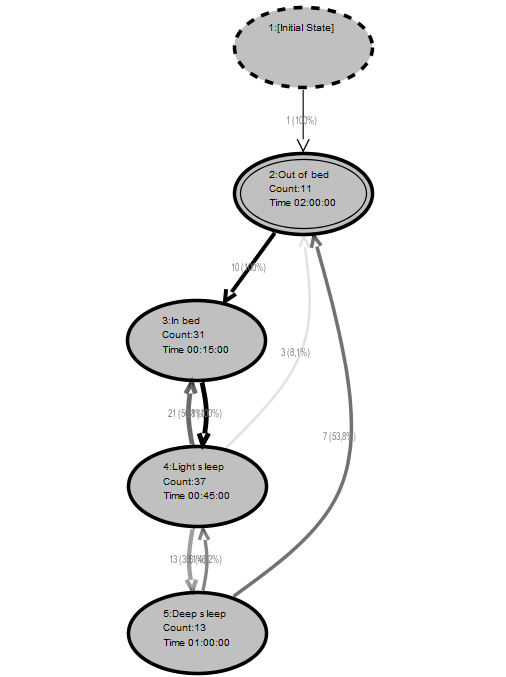
\includegraphics[width=\textwidth]{../Diagrams/sleeping.png}
        \caption{}
        \label{fig:sleeping}
    \end{subfigure}
    ~ %add desired spacing between images, e. g. ~, \quad, \qquad, \hfill etc. 
      %(or a blank line to force the subfigure onto a new line)
    \begin{subfigure}[b]{0.45\textwidth}
        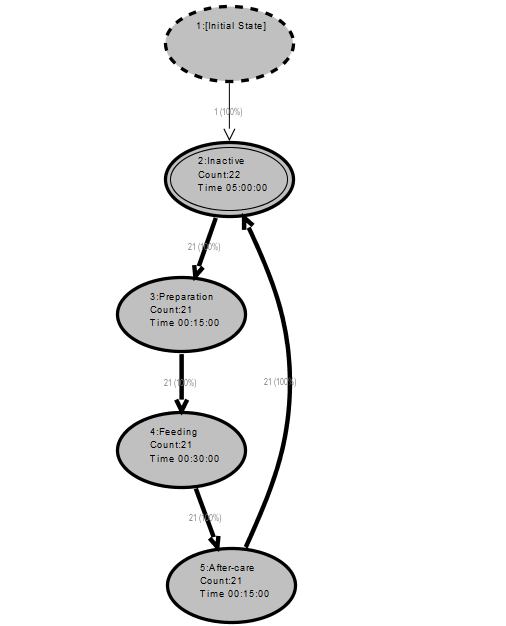
\includegraphics[width=\textwidth]{../Diagrams/feeding.png}
        \caption{}
        \label{fig:feeding}
    \end{subfigure}
    \caption{An example output for a system that is partitioned in a sleeping (\ref{fig:sleeping}) and a feeding (\ref{fig:sleeping}) cycle. The states and transitions are annotated with the statistics described in the text. The output is computed with the CSM Miner provided by the ProM tool.}
    \label{fig:exampleview}
\end{figure}

Generally, the output graphs should also illustrate the interactions between the views. A requirement taken from this might be that a click of a state in a view should mark the co-occurring states in the other views and annotate them with additional statistics of their relative frequency of co-occurrence conditioned on the number of occurrences of the clicked state. This functionality is implemented by the ProM CSM Miner. An example of such a click functionality we find in figure \ref{fig:exampleclick}.

\begin{figure}[H]
    \centering
    \begin{subfigure}[b]{0.45\textwidth}
        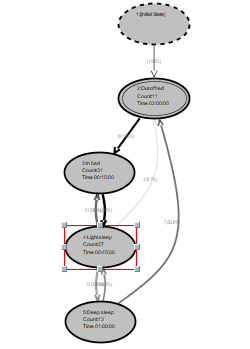
\includegraphics[width=\textwidth]{../Diagrams/sleeping_clicked.png}
        \caption{}
        \label{fig:sleep_clicked}
    \end{subfigure}
    ~ %add desired spacing between images, e. g. ~, \quad, \qquad, \hfill etc. 
      %(or a blank line to force the subfigure onto a new line)
    \begin{subfigure}[b]{0.45\textwidth}
        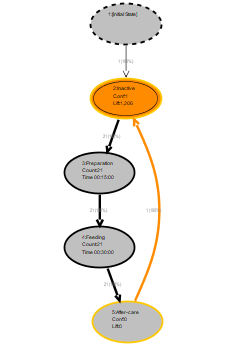
\includegraphics[width=\textwidth]{../Diagrams/feeding_marked.png}
        \caption{}
        \label{fig:feed_marked}
    \end{subfigure}
    \caption{An example click behaviour for the system introduced as an example above. In the feeding view (\ref{fig:sleep_clicked}) the state "light sleep" has been clicked. This leads to the highlighting of the two co-occurring states "inactive" and "after-care" in the feeding view (\ref{fig:feed_marked}). Also shown is information about the relative frequency of co-occurrence conditioned on the frequency of the clicked state.}
    \label{fig:exampleclick}
\end{figure}

A consultation of the advisor/client has resulted in another requirement on the click behaviour: A click in one view will result in the marking of direct and indirect successors in the other views and every such marked state is again annotated with appropriate relative frequencies.

\section{Technical Requirement}

\subsection{Needed software}
To deploy the solution there are multiple requirements. Firstly a python version greater 3 is needed. Next there is pip the software that will manage our server application. Now all we need server-wise is Django , the project was written under Django 2.2 , therefore it is recommended to use at least version 2.2.

\subsection{Client-Server architecture}
The solution requires a rather extensive client-server architecture for computational and quality of service reasons. Since the main computation is on the server the client would normally need to refresh every time a request is sent. This is not optimal for a mobile work environment since wireless networks are not as consistent as wired ones. Therefor the software only causes the client to do a complete refresh once a major computation needs to be done (e.g. create a new view), but smaller requests (e.g. labeling in current view) are computed client side. Since a project is not stored locally we will implement a request queue that will be used to handle the asynchronous work load. This queue also ensures, that a request is never lost, because an element is not deleted before the corresponding confirmation is received. 

\subsection{Django management}
To connect the front-end with the back-end Django will be used as a web server. The main tasks consist out of the following :
\begin{itemize}
	\item Receive requests and files and sent them to the back-end.
	\item Sent processed information to the client in form of a http request.
\end{itemize}

\printbibliography

\end{document}